% Class Notes Template
\documentclass[12pt]{article}
\usepackage[margin=1in]{geometry} 
\usepackage[utf8]{inputenc}

% Packages
\usepackage[french, english]{babel}
\usepackage{amsmath, amsthm, amssymb ,amsfonts, graphics, tikz, float, enumerate, graphicx}
\usepackage{listings}
\usepackage{color} %red, green, blue, yellow, cyan, magenta, black, white
\definecolor{mygreen}{RGB}{28,172,0} % color values Red, Green, Blue
\definecolor{mylilas}{RGB}{170,55,241}

\lstset{language=Matlab,%
	%basicstyle=\color{red},
	breaklines=true,%
	morekeywords={matlab2tikz},
	keywordstyle=\color{blue},%
	morekeywords=[2]{1}, keywordstyle=[2]{\color{black}},
	identifierstyle=\color{black},%
	stringstyle=\color{mylilas},
	commentstyle=\color{mygreen},%
	showstringspaces=false,%without this there will be a symbol in the places where there is a space
	numbers=left,%
	numberstyle={\tiny \color{black}},% size of the numbers
	numbersep=9pt, % this defines how far the numbers are from the text
	emph=[1]{for,end,break},emphstyle=[1]\color{blue}, %some words to emphasise
	%emph=[2]{word1,word2}, emphstyle=[2]{style},    
}

% Title
\title{ECON 6140 - Problem Set \# 3}
\date{\today}
\author{Julien Manuel Neves}

% Use these for theorems, lemmas, proofs, etc.
\newtheorem{theorem}{Theorem}
\newtheorem{corollary}[theorem]{Corollary}
\newtheorem{lemma}[theorem]{Lemma}
\newtheorem{observation}[theorem]{Observation}
\newtheorem{proposition}[theorem]{Proposition}
\newtheorem{definition}[theorem]{Definition}
\newtheorem{claim}[theorem]{Claim}
\newtheorem{fact}[theorem]{Fact}
\newtheorem{assumption}[theorem]{Assumption}
\newtheorem{problem}[theorem]{Problem}
\newtheorem{set-up}[theorem]{Set-up}
\newtheorem{example}[theorem]{Example}
\newtheorem{remark}[theorem]{Remark}
\newtheorem{axiom}[theorem]{Axiom}

% Usefuls Macros
\newcommand{\field}[1]{\mathbb{#1}}
\newcommand{\N}{\field{N}} % natural numbers
\newcommand{\R}{\field{R}} % real numbers
\newcommand{\Z}{\field{Z}} % integers
\newcommand\F{\mathcal{F}}
\newcommand\B{\mathbb{B}}
\renewcommand{\Re}{\R} % reals
\newcommand{\Rn}[1]{\mathbb{R}^{#1}}
\newcommand{\1}{{\bf 1}} % vector of all 1's
\newcommand{\I}[1]{\mathbb{I}_{\left\{#1\right\}}} % indicator function
\newcommand{\La}{\mathscr{L}}
% \newcommand{\tends}{{\rightarrow}} % arrow for limits
% \newcommand{\ra}{{\rightarrow}} % abbreviation for right arrow
% \newcommand{\subjectto}{\mbox{\rm subject to}} % subject to

%% math operators
\DeclareMathOperator*{\argmin}{arg\,min}
\DeclareMathOperator*{\argmax}{arg\,max}
\DeclareMathOperator*{\maximize}{maximize}
\DeclareMathOperator*{\minimize}{minimize}
\DeclareMathOperator{\E}{\mathsf{E}} % expectation
\newcommand{\Ex}[1]{\E\left\{#1\right\}} % expectation with brackets
\DeclareMathOperator{\pr}{\mathsf{P}} % probability
\newcommand{\prob}[1]{\pr\left\{#1\right\}}
\DeclareMathOperator{\subjectto}{{s.t.\ }} % subject to
\newcommand{\norm}[1]{\left\|#1\right\|}
\newcommand{\card}[1]{\left|#1\right|}

% Extra stuff
\newcommand\seq[1]{\{ #1 \}}
\newcommand{\inp}[2]{\langle #1, #2 \rangle}

\newcommand{\inv}{^{-1}}

\newcommand{\pa}[1]{\left(#1\right)}
\newcommand{\bra}[1]{\left[#1\right]}
\newcommand{\cbra}[1]{\left\{ #1 \right\}}

\newcommand{\pfrac}[2]{\pa{\frac{#1}{#2}}}
\newcommand{\bfrac}[2]{\bra{\frac{#1}{#2}}}

\newcommand{\mat}[1]{\begin{matrix}#1\end{matrix}}
\newcommand{\pmat}[1]{\pa{\mat{#1}}}
\newcommand{\bmat}[1]{\bra{\mat{#1}}}

\begin{document}

\maketitle

\section*{Open Economy with Durable Goods}

\begin{enumerate}[(1)]
	\item 
	
	The Langrangian of the problem:
	\begin{align*}
	\mathcal{L} = \sum_{t=0}^{\infty}\beta^t[u(c_t)+v(z_{t+1}) &+\lambda_t(R^*b_t+af(k_t)-c_t-x_{kt}-qx_{zt}-b_{t+1}-\frac{d}{2}(z_{t+1}-z_t)^2) \\
	&+\mu_t(x_{zt}+(1-\delta_z)z_t-z_{t+1})\\
	&+\nu_t(x_{kt}+(1-\delta_k)k_t-k_{t+1}) ]
	\end{align*}
	
	KKT:
	\begin{align*}
	c_{t}&: c_t^{-\eta}-\lambda_t=0\\
	z_{t+1}&:z_{t+1}^{-\eta}-\lambda_td(z_{t+1}-z_t)+\beta \lambda_{t+1}d(z_{t+2}-z_{t+1})-\mu_t+ \beta \mu_{t+1} (1-\delta_z) =0\\
	b_{t+1}&: \beta \lambda_{t+1}R^* - \lambda_t =0\\
	k_{t+1}&:\beta \lambda_{t+1} a f'(k_{t+1}) + \beta \nu_{t+1}(1-\delta_k) -\nu_t=0 \\
	x_{zt}&:\mu_t-q\lambda_t  =0 \\
	x_{kt}&:\nu_t-\lambda_t  =0\\
	&:R^*b_t+af(k_t)\geq c_t+x_{kt}+qx_{zt}+b_{t+1}+\frac{d}{2}(z_{t+1}-z_t)^2\\
	&:x_{zt}+(1-\delta_z)z_t\geq z_{t+1}\\
	&:x_{kt}+(1-\delta_k)k_t\geq k_{t+1}\\
	TVC_1&:\lim_{T\to \infty}\beta^Tu_c(c_T)k_{T+1}  =0\\
	TVC_2&:\lim_{T\to \infty}\beta^Tu_c(c_T)b_{T+1}  =0
	\end{align*}
	
	Note that we need an extra tranversality condition for capital.
	
	
	Note that since $R^*=\frac{1}{\beta}$, then $\lambda_t = \lambda_{t+1}$.
	
	The steady state FOCs are given by
			\begin{align*}
	&\left( \frac{c}{z}\right) ^{\eta} = q(1-\beta(1-\delta_z))\\
	&\beta(af'(k)+(1-\delta_k))=1
	\end{align*}
	and the steady state constraint yield
		\begin{align*}
	&(R^*-1)b+af(k)= c+x_{k}+qx_{z}\\
	&x_{z}=\delta_zz\\
	&x_{k}= \delta_zk
	\end{align*}

Note that if $f'(\cdot)$ is decreasing, $k$ is uniquely determined by $(\beta,a,\delta_k,f(\cdot))$.

Since $d$ doesn't enter these equations, hence it is irrelevant for the steady states.

If $q\uparrow$ or $\delta_z \uparrow$, then $\frac{c}{z} \uparrow$. Since $k$ is only determined by the coefficient, we need $b$ to adjust such that $(R^*-1)b+af(k)= c+q\delta_zz+\delta_zk$ holds for the new steady state.
	
	\item 
	
	Recall that since $R^*=\frac{1}{\beta}$, we have $\lambda_t = \lambda_{t+1} = \lambda$. This in turns implies that 
	$\mu_t=q\lambda$ and $\nu_t=\lambda$, i.e. every Lagrange multiplier is constant. This implies that $c_t$ and $z_{t+1}$ are also constant for $t\geq 0$. Note that $z_0$ is given, therefore $z_t=z$ for $t\geq 1$ which might not be equal to $z_0$. In fact, $z$ is equal to the steady state value of 
	\[
	z= c[q(1-\beta(1-\delta_z))]^{-\frac{1}{\eta}}
	\]
	
	Moreover, we get
	\[
	\beta(af'(k_{t+1})+(1-\delta_k))=1
	\]
	i.e. $k_{t+1}$ is also constant if $f'(\cdot)$ is decreasing and $k$ is given by $\beta(af'(k)+(1-\delta_k))=1$.
	
	Since $k_{t+1}$ is constant $x_{kt}+(1-\delta_k)k_t= k_{t+1}$ becomes $x_{kt}=\delta_kk$ for $t\geq 1$ and $x_{k0}=k-(1-\delta_k)k_0$ for $t=0$.
	Since $z_{t+1}$ is constant $x_{zt}+(1-\delta_z)z_t= z_{t+1}$ becomes $x_{zt}=\delta_zz$ for $t\geq 1$ and $x_{z0}=z-(1-\delta_z)z_0$ for $t=0$.
	
	Now, we look at the dynamics of $b_t$. Note that it is fully determined by
	\[
	b_{t+1}=R^*b_t+af(k_t)- c-x_{kt}-qx_{zt}
	\]
	Since we know $b_0$, the whole sequence of $x_{kt}$ and $x_{zt}$, the only thing missing is $c$. As shown previously, $c_t$ is constant. Hence, to pin down $b_t$ we need to find $c_0=c$.
	
	Let's look at the phase diagram of $b$ and $z$ with $t\geq 1$. Note that we get the following equation
\begin{align*}
	z_{t+1} = z_t = z\\
	b_{t+1}=R^*b_t+af(k)- c-\delta_k k-q\delta_z z_t
\end{align*}

Hence, the locus for $b$ is
\begin{align*}
	b_{t}=-\frac{a\beta}{1-\beta}f(k)+ \frac{c\beta}{1-\beta}+ \frac{\delta_k\beta}{1-\beta}k+\frac{q\delta_z\beta}{1-\beta} z_t
\end{align*}

Hence, the steady state is $b=-\frac{a\beta}{1-\beta}f(k)+ \frac{c\beta}{1-\beta}+ \frac{\delta_k\beta}{1-\beta}k+\frac{q\delta_z\beta}{1-\beta} z$. Since $z_t$ is constant, to get to the steady state, we need $b_t=b$. Therefore, we need $c$ to be such that $b_1 = -\frac{a\beta}{1-\beta}f(k)+ \frac{c\beta}{1-\beta}+ \frac{\delta_k\beta}{1-\beta}k+\frac{q\delta_z\beta}{1-\beta} z$.

Hence, we choose $c_0=c$ such that $b_{1}=R^*b_0+af(k_0)- c_0-x_{k0}-qx_{z0}$ holds and voil\`a!

	\item 
	
	Again, every Lagrange multiplier are constant. Therefore, we get
	\[
	\beta(af'(k_{t+1})+(1-\delta_k))=1
	\]
	i.e. $k_{t+1}$ is constant if $f'(\cdot)$ is decreasing. Since $k_{t+1}$ is constant $x_{kt}+(1-\delta_k)k_t= k_{t+1}$ becomes $x_{kt}=\delta_kk$ for $t\geq 1$ and $x_{k0}=k-(1-\delta_k)k_0$ for $t=0$.
	
	Moreover, the FOC of $z_{t+1}$ is now
	\[
	z_{t+1}^{-\eta}= \lambda [d(z_{t+1}-z_t)-\beta d(z_{t+2}-z_{t+1})+q(1- \beta (1-\delta_z) )]
	\]
	
	Since capital is constant, we can focus on a phase diagram to see what happens to $z_t$ only. Let $y_t= z_{t+1}-z_t$. Hence, we have the two following dynamic equations
	\begin{align*}
		z_{t+1} & = y_t + z_t\\
	y_{t+1}&= \frac{1}{\beta }y_{t} + \frac{q}{\beta d}(1- \beta (1-\delta_z) ) -\frac{1}{\lambda \beta d}(y_{t}+z_{t})^{-\eta}
	\end{align*}
	
	Take the loci where $z$ is constant. This yields $y=0$, i.e. the $y$-axis.
	
	For the second loci is shape is not too important for our analysis. We simply note that for $y=0$, we get
	\[
		z ^{-\eta} = \lambda q(1-\beta(1-\delta_z))
	\]
	Since, $\lambda = c^{-\eta}$, we have $z ^{-\eta} = c^{-\eta} q(1-\beta(1-\delta_z))$, i.e. the steady state derived previously.
	
	To describe the dynamics, take $y_t<0$. This implies that $z_{t+1}<z_t$. Therefore on the steady path, if we start over the steady state, $z_t$ will decrease until it reaches $z$. The reverse can be said for $y_t>0$. The speed of converge is describe in part 4).

	\item 
	
	Note that as derived previously, capital goods are constant for period $t\geq 1$. Hence to converge to the steady state, we only one period.
	
	For durable goods, our analysis implies that regardless if we start over or under the second locus, the $y_t$ will converge to the steady state $y=0$ over time. This in turns implies that the difference between $z_{t+1}$ and $z_{t}$ will decrease every period until $z_t=z$. Hence, the convergence of durable goods is not ``instantaneous'' like capital.
\end{enumerate}
	
	
	\section*{Transition paths in the one sector growth model}
	
	\begin{enumerate}[(1)]
		\item 
		
		With the parameters defined in the problem set, we get that the steady state is $k^*=10.03 $ and $c^*=1.639$. Thus, our starting value is $k_0 = 9.027599$. Figure \ref{fig:fig1} shows the transition of $k_0$ on the steady path. It takes $53$ periods to converge to the steady state when starting from $k_0=.9k^*$.

		\begin{figure}[H]
	\centering
	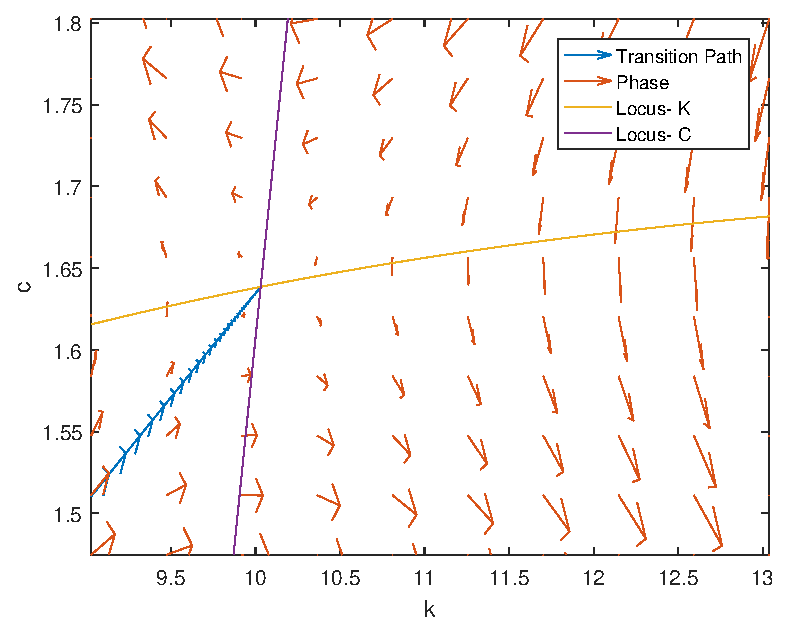
\includegraphics[width=0.7\linewidth]{fig1}
	\caption{Transition path for growth model starting at $k_0=.9k^*$}
	\label{fig:fig1}
\end{figure}

Note that we also plot the loci of our phase diagram on Figure \ref{fig:fig1}. Recall that they are given by
\begin{align*}
	k:& c_t =Ak_t^\alpha - \delta k_t   \\
	c:& c_t = k_t^\alpha +(1-\delta)k_t-k^*
\end{align*}
where $k^*$ is the steady state value equal to $\left( \frac{\alpha\beta A}{1-\beta+\beta\delta}\right)^\frac{1}{1-\alpha}$.

		
		\item 
		See Figure \ref{fig:fig2}.
				\begin{figure}[H]
			\centering
			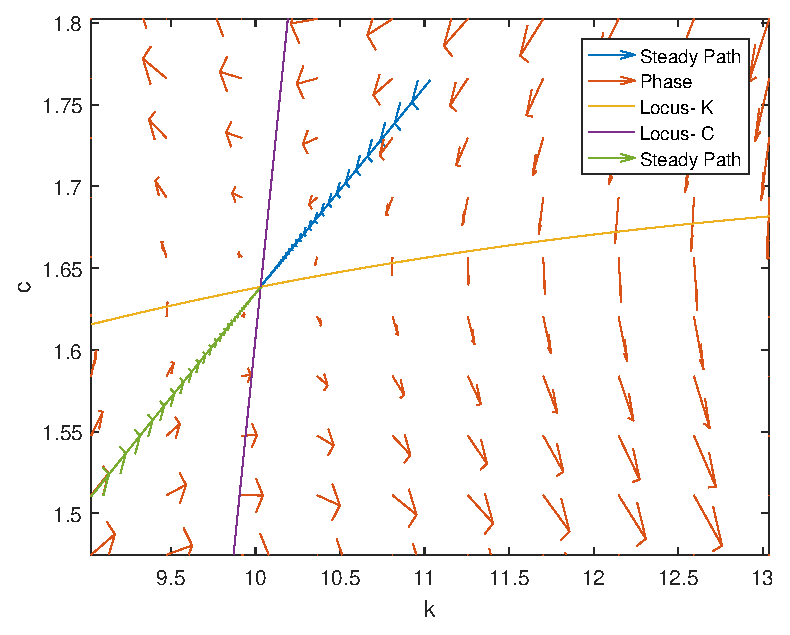
\includegraphics[width=0.7\linewidth]{fig2}
			\caption{Phase diagram for growth model}
			\label{fig:fig2}
		\end{figure}
		 Note that the scales on this figure are not 1-1.
		\item 
				\begin{figure}[H]
			\centering
			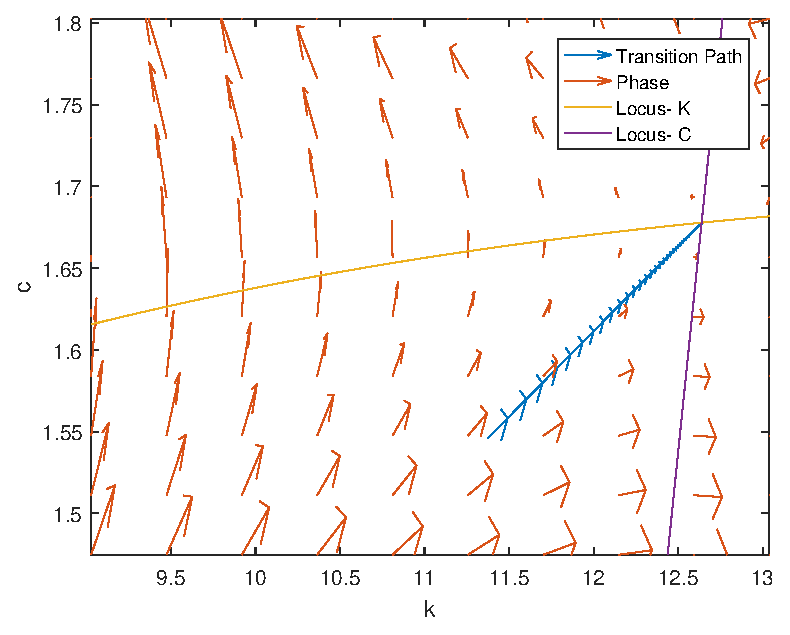
\includegraphics[width=0.7\linewidth]{fig3}
			\caption{Phase diagram for growth model with increase of 1\% in $\beta$}
			\label{fig:fig3}
		\end{figure}
By increasing $\beta$ by 1\% the second locus shift to the right and we get that the new steady state is $k^*=12.640$ and $c^*=1.678$. Therefore the starting value is $k_0 = 11.376$. Note that since $k^*$ is bigger, $k_0$ is a bit farther in absolute terms. This results in a longer convergence term of $59$ periods. The transition path is plotted in Figure \ref{fig:fig3}.


		\item 
		
		Note that if $A$ goes up, the first locus also goes up. This implies that the new steady path also shifts up and the new steady state will be one where $k^*\uparrow$ and $c^*\uparrow$. 
		
		In this problem, we let the increase in $A$ happen at $t=1$. Moreover, let's assume that it was an unexpected increase permanent increase in $A$, i.e. consumer don't preventively adjust to a future steady path.
						\begin{figure}[H]
			\centering
			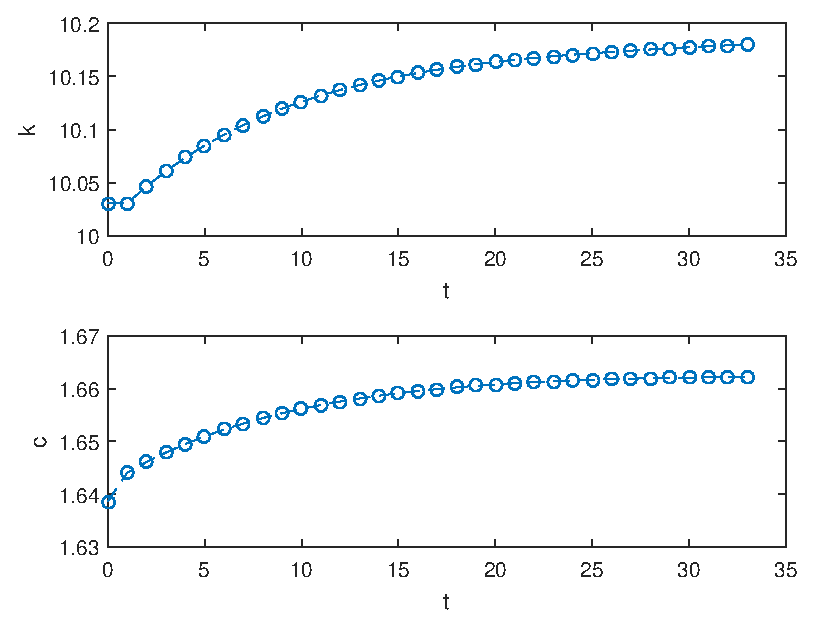
\includegraphics[width=0.7\linewidth]{fig4}
			\caption{Time path for consumption and capital with increase of 1\% in $A$}
			\label{fig:fig4}
		\end{figure}
		
		Now, since the point $(k_0,c_0)$ is the old steady , it might not be on the new steady path. To adjust to that the consumer will instantaneously change it consumption at time $t=1$ to get on the new steady path unlike $k_0$ that can't act reactively. From there on on out, both $k_t$ and $c_t$ will monotonically increase until it reaches the new steady path as shown in Figure \ref{fig:fig4}. 
	\end{enumerate}

\section*{Code}

\lstinputlisting[language=Matlab]{shooting.m}

\end{document}
